\section{Graphical Notation and Figure Conventions}

The diagrams in this document are designed to show how tensors flow through a Transformer layer and its parallel variants. This section summarizes the graphical notation, including tensor-shape labels, node types, edge styles, and the small operator dictionary for the most common nodes (matmul, softmax, scale/mask, dropout, layer normalization, communication, and broadcast).

Throughout the figures, the goal is to emphasize the flow of tensors along edges. The exact Jacobian matrices for each operation are not drawn; instead, the backward nodes are understood as the abstract operators $\mathrm{d}f$ introduced in Section 3.

\subsection{Tensor Shapes and Index Notation}

We use a consistent braced notation for tensor shapes. Instead of writing $\mathbb{R}^{B \times S \times D}$, we annotate edges in the diagrams with labels such as
\[
[B, S, D], \quad [B, N_H, S, D_h], \quad [D, D_{ff}],
\]
directly next to the arrows. This makes it easier to match each edge to a particular dimension ordering.

The main symbols are:
\begin{itemize}
\item $B$: batch size.
\item $S$: sequence length (number of tokens per sequence).
\item $D$: model (hidden) dimension.
\item $D_{ff}$: intermediate MLP (feed-forward) dimension.
\item $N_H$: number of attention heads.
\item $D_h$: per-head dimension, typically $D_h = D/N_H$.
\end{itemize}

Typical tensor shapes in the diagrams include:
\begin{itemize}
\item $\mathbf{X} \in [B, S, D]$: input or hidden states.
\item $\mathbf{H} \in [B, S, D]$: normalized or intermediate states.
\item $\mathbf{Q}, \mathbf{K}, \mathbf{V} \in [B, N_H, S, D_h]$: projected queries, keys, and values.
\item $\mathbf{AS} \in [B, N_H, S, S]$: attention scores after scaling/masking and softmax.
\item $\mathbf{Y} \in [B, S, D]$: output of a Transformer block or layer.
\end{itemize}

Under tensor parallelism (TP) and data parallelism (DP) we mostly keep the same shape notation on edges. For example, a TP shard that actually stores a slice of width $D/N_T$ may still be labeled $[B, S, D]$ in an end-to-end figure when we want to focus on the logical model dimension rather than the physical shard size. When necessary, shard dimensions such as $[B, S, D/N_T]$ or $[B, N_H/N_T, S, D_h]$ are written explicitly.

Gradients use the same shape conventions. For example:
\[
\mathrm{d}\mathbf{X} \in [B, S, D], \quad \mathrm{d}\mathbf{W}_Q \in [D, D], \quad \mathrm{d}\mathbf{W}_{\text{up}} \in [D, D_{ff}].
\]

\subsection{Nodes, Edges, and Arrow Styles}

The diagrams are drawn as computation graphs. Nodes represent local operations; edges represent tensors flowing between them.

\subsubsection{Forward vs. Backward Arrows}

We distinguish between forward and backward flows:
\begin{itemize}
\item \textbf{Overall flow diagrams} (e.g. the top-level Transformer flow) use:
  \begin{itemize}
  \item solid arrows for forward activations (e.g. $\mathbf{X}$ to $\mathbf{Y}$);
  \item dashed arrows for backward gradients (e.g. $\mathrm{d}\mathbf{Y}$ to $\mathrm{d}\mathbf{X}$).
  \end{itemize}
\item \textbf{Detailed backward diagrams} (e.g. MHA backward, MLP backward) use thicker arrows with different styles (single vs. double) to distinguish:
  \begin{itemize}
  \item gradient flow along the main backward path,
  \item cached forward values reused as secondary inputs to backward nodes.
  \end{itemize}
\end{itemize}

In all cases, the arrow direction follows the direction of computation for forward edges and the direction of gradient propagation for backward edges.

\subsubsection{Node Types}

We use a small set of recurring node types:

\paragraph{Matrix multiplication.} A matrix multiplication node is drawn as a circle containing a dot:
\[
\bullet
\]
In the forward pass this corresponds to an operation such as $\mathbf{Y} = \mathbf{X}\mathbf{W}$. In the backward diagrams the corresponding dNode (e.g. \texttt{dMatmul}) implements the abstract backward operator
\[
(\mathrm{d}\mathbf{X}, \mathrm{d}\mathbf{W}) = \mathrm{d}f(\mathbf{X}, \mathbf{W}, \mathrm{d}\mathbf{Y}),
\]
as described in Section 3.

\paragraph{Addition and residuals.} Elementwise addition is drawn as a circle containing a plus:
\[
+
\]
This is used for bias addition, combining residual connections, and aggregating multiple gradient contributions. Small circles labeled $\sum$ denote explicit summations over batch and/or sequence dimensions (e.g. $\sum_{B,S}$ for bias-gradient accumulation).

\paragraph{Generic rectangular operators.} Many local operations (layer normalization, nonlinearity, dropout, scale/mask, reshape, transpose) are drawn as rectangles with short labels such as \texttt{LN}, \texttt{GL}, \texttt{DO}, \texttt{SM}, \texttt{R}, or \texttt{T}. Their backward counterparts are labeled with a leading ``d'', for example \texttt{dLN}, \texttt{dDO}, \texttt{dSM}. Each such dNode implements the corresponding backward operator $\mathrm{d}f(\cdot, \ldots, \cdot, \mathrm{d}\mathbf{y})$.

\paragraph{Communication nodes.} Distributed communication collectives are drawn as small rectangular nodes with labels such as:
\begin{itemize}
\item \texttt{AR}: All-Reduce.
\item \texttt{AG}: All-Gather.
\end{itemize}
The arrows entering/leaving these nodes indicate which tensors are participating in the collective, and the shape annotations show the logical tensor size before and after the communication.

\subsection{Forward and Backward Nodes: Abstract View}

Most operators in a Transformer layer can be written abstractly as
\[
\mathbf{y} = f(\mathbf{x}_1, \ldots, \mathbf{x}_k),
\]
where $\mathbf{x}_1, \ldots, \mathbf{x}_k$ include both activations and parameters (such as weight matrices or bias vectors). In Section 3 we introduced the abstract backward operators
\[
\mathrm{d}\mathbf{x}_i = \mathrm{d}_{\mathbf{x}_i}f(\mathbf{x}_1, \ldots, \mathbf{x}_k, \mathrm{d}\mathbf{y}), \quad i = 1, \ldots, k.
\]

\textbf{How to read nodes in our diagrams:}

\begin{center}
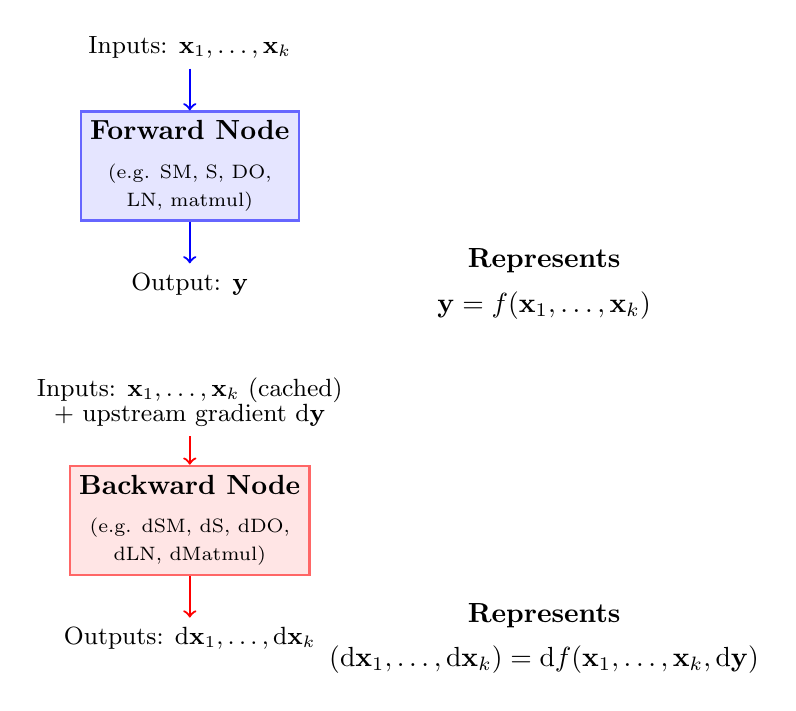
\begin{tikzpicture}[
  node distance=2.5cm,
  fwdnode/.style={rectangle, draw=blue!60, fill=blue!10, thick, minimum width=1.8cm, minimum height=1cm, align=center},
  bwdnode/.style={rectangle, draw=red!60, fill=red!10, thick, minimum width=1.8cm, minimum height=1cm, align=center},
  arrow/.style={->, thick},
  label/.style={font=\small}
]

% Forward node
\node[fwdnode] (fwd) {\textbf{Forward Node}\\[2pt]\scriptsize (e.g. SM, S, DO,\\[-2pt]\scriptsize LN, matmul)};

\node[above of=fwd, node distance=1.5cm, label] (fwd_in) {Inputs: $\mathbf{x}_1, \ldots, \mathbf{x}_k$};
\node[below of=fwd, node distance=1.5cm, label] (fwd_out) {Output: $\mathbf{y}$};

\draw[arrow, blue] (fwd_in) -- (fwd);
\draw[arrow, blue] (fwd) -- (fwd_out);

\node[right of=fwd_out, node distance=4.5cm, align=center] (fwd_eq) {
  \textbf{Represents}\\[4pt]
  $\mathbf{y} = f(\mathbf{x}_1, \ldots, \mathbf{x}_k)$
};

% Backward node
\node[bwdnode, below of=fwd, node distance=4.5cm] (bwd) {\textbf{Backward Node}\\[2pt]\scriptsize (e.g. dSM, dS, dDO,\\[-2pt]\scriptsize dLN, dMatmul)};

\node[above of=bwd, node distance=1.5cm, label, align=center] (bwd_in) {Inputs: $\mathbf{x}_1, \ldots, \mathbf{x}_k$ (cached)\\[-2pt] + upstream gradient $\mathrm{d}\mathbf{y}$};
\node[below of=bwd, node distance=1.5cm, label] (bwd_out) {Outputs: $\mathrm{d}\mathbf{x}_1, \ldots, \mathrm{d}\mathbf{x}_k$};

\draw[arrow, red] (bwd_in) -- (bwd);
\draw[arrow, red] (bwd) -- (bwd_out);

\node[right of=bwd_out, node distance=4.5cm, align=center] (bwd_eq) {
  \textbf{Represents}\\[4pt]
  $(\mathrm{d}\mathbf{x}_1, \ldots, \mathrm{d}\mathbf{x}_k) = \mathrm{d}f(\mathbf{x}_1, \ldots, \mathbf{x}_k, \mathrm{d}\mathbf{y})$
};

\end{tikzpicture}
\end{center}

\vspace{0.3cm}

In the diagrams:
\begin{itemize}
\item A \textbf{forward node} (e.g. \texttt{S}, \texttt{SM}, \texttt{DO}, \texttt{LN}, \texttt{matmul}) represents the mapping $\mathbf{y} = f(\mathbf{x}_1, \ldots, \mathbf{x}_k)$.
\item The corresponding \textbf{backward node} (labeled with a leading ``d'', e.g. \texttt{dS}, \texttt{dSM}, \texttt{dDO}, \texttt{dLN}) represents the mapping
\[
(\mathrm{d}\mathbf{x}_1, \ldots, \mathrm{d}\mathbf{x}_k) = \mathrm{d}f(\mathbf{x}_1, \ldots, \mathbf{x}_k, \mathrm{d}\mathbf{y}),
\]
i.e. it consumes the upstream gradient $\mathrm{d}\mathbf{y}$ and the necessary cached forward inputs, and produces gradients for all inputs.
\end{itemize}

The purpose of this section is not to re-derive all Jacobian formulas, but to provide a dictionary that tells the reader what each node means in the diagrams and how to read its inputs/outputs at the level of tensors and gradients.

\subsection{Operator Dictionary: Forward and Backward}

We now describe the most common node types used in the MHA, MLP, and output-projection diagrams. For each operator we briefly summarize the forward computation and the corresponding backward operator in the abstract notation $\mathrm{d}f(\cdot, \ldots, \cdot, \mathrm{d}\mathbf{y})$.

\subsubsection{Matrix Multiplication (Matmul)}

\textbf{Forward.} A matmul node computes
\[
\mathbf{Y} = \mathbf{X}\mathbf{W},
\]
with shapes such as $\mathbf{X} \in [B, S, D]$, $\mathbf{W} \in [D, D]$, and $\mathbf{Y} \in [B, S, D]$. The same pattern appears in the MLP block with $\mathbf{W}_{\text{up}} \in [D, D_{ff}]$ or $\mathbf{W}_{\text{down}} \in [D_{ff}, D]$.

\textbf{Backward.} The backward node \texttt{dMatmul} implements
\[
(\mathrm{d}\mathbf{X}, \mathrm{d}\mathbf{W}) = \mathrm{d}f(\mathbf{X}, \mathbf{W}, \mathrm{d}\mathbf{Y}),
\]
with the usual formulas
\[
\mathrm{d}\mathbf{X} = \mathrm{d}\mathbf{Y}\mathbf{W}^T, \quad \mathrm{d}\mathbf{W} = \mathbf{X}^T \mathrm{d}\mathbf{Y},
\]
applied with appropriate reshaping for batched tensors. In the diagrams, $\mathbf{X}$ and $\mathbf{W}$ (or their transposes) are supplied to the \texttt{dMatmul} node via double arrows, and outgoing arrows carry $\mathrm{d}\mathbf{X}$ and $\mathrm{d}\mathbf{W}$.

\subsubsection{Broadcast (BC)}

In many diagrams we annotate bias addition by a term such as $\text{BC}_{B,S}(\mathbf{b}_0)$, which denotes a logical broadcast of a 1-D bias vector $\mathbf{b}_0 \in [D]$ or $[D_{ff}]$ across the batch and sequence dimensions to match a tensor of shape $[B, S, D]$ or $[B, S, D_{ff}]$.

\textbf{Forward.} Conceptually,
\[
\mathbf{Y} = \mathbf{X} + \text{BC}_{B,S}(\mathbf{b}_0),
\]
where $\text{BC}_{B,S}(\mathbf{b}_0)$ is a tensor in $[B, S, D]$ obtained by repeating $\mathbf{b}_0$ over the $B$ and $S$ dimensions. In the diagrams we typically draw only the addition node and label the edge near the bias with $\text{BC}_{B,S}(\mathbf{b}_0)$ to indicate that the bias is broadcast in this way.

\textbf{Backward.} The backward contribution to $\mathrm{d}\mathbf{b}_0$ is obtained by summing $\mathrm{d}\mathbf{Y}$ over the broadcast dimensions:
\[
\mathrm{d}\mathbf{b}_0 = \sum_{b=1}^B \sum_{s=1}^S \mathrm{d}\mathbf{Y}_{b,s,:},
\]
which is represented in the diagrams by a small summation node labeled $\sum_{B,S}$. The gradient $\mathrm{d}\mathbf{X}$ simply inherits $\mathrm{d}\mathbf{Y}$, since the addition is symmetric.

\subsubsection{Scale/Mask Node (SM, dSM)}

In the attention mechanism, raw scores $\mathbf{A}$ from $\mathbf{Q}\mathbf{K}^T$ are scaled and masked before softmax. This is represented by a node labeled \texttt{SM} (scale/mask).

\textbf{Forward (SM).} Given attention scores $\mathbf{A} \in [B, N_H, S, S]$, the \texttt{SM} node computes
\[
\mathbf{Z} = \text{SM}(\mathbf{A}) = \alpha \mathbf{A} + \mathbf{M},
\]
where $\alpha = 1/\sqrt{D_h}$ is a scalar and $\mathbf{M}$ encodes the mask (e.g. large negative values at disallowed positions). The shape of $\mathbf{Z}$ matches $\mathbf{A}$. The forward pass caches the scaling factor and the mask pattern.

\textbf{Backward (dSM).} The backward node \texttt{dSM} is the abstract operator
\[
\mathrm{d}\mathbf{A} = \mathrm{d}\text{SM}(\mathbf{A}, \mathrm{d}\mathbf{Z}),
\]
with
\[
\mathrm{d}\text{SM}(\mathbf{A}, \mathrm{d}\mathbf{Z}) = \alpha \, \mathrm{d}\mathbf{Z},
\]
and no gradient is propagated into the fixed mask $\mathbf{M}$. In the diagram, $\mathbf{A}$ and $\mathrm{d}\mathbf{Z}$ enter the \texttt{dSM} node, and $\mathrm{d}\mathbf{A}$ exits as the gradient with respect to the raw attention scores.

\subsubsection{Softmax Node (S, dS)}

The node labeled \texttt{S} performs softmax over the key dimension of the attention scores.

\textbf{Forward (S).} For a fixed batch $b$, head $h$, and query position $s$, let $\mathbf{z} \in \mathbb{R}^S$ be the vector of scores over keys. Softmax produces
\[
\mathbf{p} = \text{softmax}(\mathbf{z}), \quad p_i = \frac{e^{z_i}}{\sum_j e^{z_j}}.
\]
This is applied to every $(b, h, s)$, so the overall shape $[B, N_H, S, S]$ is preserved. The forward pass typically caches $\mathbf{p}$ (or $\mathbf{z}$).

\textbf{Backward (dS).} The backward node \texttt{dS} implements the local mapping
\[
\mathrm{d}\mathbf{z} = \mathrm{d}\text{S}(\mathbf{z}, \mathrm{d}\mathbf{p}),
\]
which, in Jacobian form, is
\[
\mathrm{d}\text{S}(\mathbf{z}, \mathrm{d}\mathbf{p}) = \mathbf{J}_{\text{softmax}}(\mathbf{z})^T \mathrm{d}\mathbf{p}.
\]
In practice this is computed using the standard softmax backward formula. In the diagrams, the \texttt{dS} node has incoming edges carrying $\mathbf{p}$ (or $\mathbf{z}$) and $\mathrm{d}\mathbf{p}$, and an outgoing edge carrying $\mathrm{d}\mathbf{z}$.

\subsubsection{Nonlinearities and Dropout (GL, dGL, DO, dDO)}

Rectangular nodes labeled \texttt{GL}, \texttt{GELU}, or similar denote elementwise nonlinearities; nodes labeled \texttt{DO} denote dropout.

\textbf{Forward (GL / DO).} For a generic scalar nonlinearity $g$,
\[
\mathbf{Y} = g(\mathbf{X})
\]
is applied elementwise. For dropout we write
\[
\mathbf{Y} = \text{DO}(\mathbf{X}; \mathbf{m}) = \mathbf{m} \odot \mathbf{X},
\]
where $\mathbf{m}$ is a binary mask of the same shape as $\mathbf{X}$ and $\odot$ denotes elementwise multiplication. The mask $\mathbf{m}$ is cached in the forward pass.

\textbf{Backward (dGL / dDO).} For a generic nonlinearity, the backward node \texttt{dGL} implements
\[
\mathrm{d}\mathbf{X} = \mathrm{d}\text{GL}(\mathbf{X}, \mathrm{d}\mathbf{Y}) = \mathrm{d}\mathbf{Y} \odot g'(\mathbf{X}),
\]
using the forward input $\mathbf{X}$ from the cache.

For dropout, the backward node \texttt{dDO} implements
\[
\mathrm{d}\mathbf{X} = \mathrm{d}\text{DO}(\mathbf{X}, \mathrm{d}\mathbf{Y}) = \mathbf{m} \odot \mathrm{d}\mathbf{Y}.
\]
In the diagrams, the node labeled \texttt{dDO} consumes the upstream gradient $\mathrm{d}\mathbf{Y}$ and the cached mask $\mathbf{m}$, and produces $\mathrm{d}\mathbf{X}$.

\subsubsection{Layer Normalization (LN, dLN)}

Layer normalization nodes are labeled \texttt{LN} in the forward pass and \texttt{dLN} in the backward pass.

\textbf{Forward (LN).} Given $\mathbf{X} \in [B, S, D]$, layer normalization computes
\[
\mathbf{H} = \text{LN}(\mathbf{X}; \gamma, \beta),
\]
by normalizing each $[D]$-dimensional vector at fixed $B, S$, and applying learned scale and shift parameters $\gamma, \beta \in [D]$. The forward pass caches per-position mean/variance as well as $\gamma$ and $\beta$.

\textbf{Backward (dLN).} The backward node \texttt{dLN} implements
\[
(\mathrm{d}\mathbf{X}, \mathrm{d}\gamma, \mathrm{d}\beta) = \mathrm{d}\text{LN}(\mathbf{X}, \gamma, \beta, \mathrm{d}\mathbf{H}, \text{stats}),
\]
where $\text{stats}$ denotes the cached means and variances. The explicit formulas follow from the standard layer-normalization backward derivation; in the diagrams we treat \texttt{dLN} as a single node that consumes $\mathbf{X}$, $\gamma$, the cached statistics, and $\mathrm{d}\mathbf{H}$, and produces three outgoing gradient edges $\mathrm{d}\mathbf{X}$, $\mathrm{d}\gamma$, and $\mathrm{d}\beta$.

\subsubsection{Communication Nodes (AR, AG)}

In tensor-parallel (TP), data-parallel (DP), and hybrid DP+TP settings, collective communication operations synchronize tensors across devices.

\textbf{All-Reduce (AR).} An All-Reduce node \texttt{AR} takes as input a tensor shard from each participant and outputs the elementwise reduced tensor (typically a sum), optionally divided by the number of participants for averaging. For example, in DP, weight gradients $\mathrm{d}\mathbf{W}$ of shape $[D, D]$ are All-Reduced across all data-parallel ranks before the optimizer step.

\textbf{All-Gather (AG).} An All-Gather node \texttt{AG} concatenates or aggregates tensor shards across a parallel group to reconstruct a full tensor. For example, in TP, partial outputs along a hidden dimension may be gathered to form a full $[B, S, D]$ tensor.

In the diagrams, these communication nodes are treated as pure operators on tensors; their backward behavior (e.g. gradient flow through \texttt{AR} and \texttt{AG}) is implicit in the symmetry of the operations.

\subsection{Reading the Detailed MHA and MLP Figures}

With the conventions above, the large MHA and MLP forward/backward figures can be read as follows:
\begin{itemize}
\item \textbf{Edges} indicate the flow of tensors (activations or gradients), annotated with shapes like $[B, S, D]$ or $[B, N_H, S, D_h]$.
\item \textbf{Forward nodes} (\texttt{S}, \texttt{SM}, \texttt{DO}, \texttt{LN}, \texttt{matmul}, \texttt{reshape}, \texttt{transpose}) compute local functions $f(\mathbf{x}_1, \ldots, \mathbf{x}_k)$.
\item \textbf{Backward nodes} (\texttt{dS}, \texttt{dSM}, \texttt{dDO}, \texttt{dLN}, \texttt{dMatmul}) implement the corresponding backward operators $\mathrm{d}f(\mathbf{x}_1, \ldots, \mathbf{x}_k, \mathrm{d}\mathbf{y})$, producing gradients for all inputs.
\item \textbf{Broadcast labels} such as $\text{BC}_{B,S}(\mathbf{b}_0)$ indicate that a bias vector is conceptually expanded to match a higher-rank tensor before addition.
\item \textbf{Communication nodes} (\texttt{AR}, \texttt{AG}) indicate where collective operations occur in TP, DP, or DP+TP settings, and their shape annotations show the logical dimensions involved.
\end{itemize}

These conventions allow the reader to understand the data and gradient flows at a glance, without being distracted by low-level indexing, while still being precise enough to derive the underlying equations when needed.
